%%%%%%%%%%%%%%%%%%%%%%%%%%%%%%%%%%%%%%%%%
% Beamer Presentation
% LaTeX Template
% Version 1.0 (10/11/12)
%
% This template has been downloaded from:
% http://www.LaTeXTemplates.com
%
% License:
% CC BY-NC-SA 3.0 (http://creativecommons.org/licenses/by-nc-sa/3.0/)
%
%%%%%%%%%%%%%%%%%%%%%%%%%%%%%%%%%%%%%%%%%

%----------------------------------------------------------------------------------------
%	PACKAGES AND THEMES
%----------------------------------------------------------------------------------------

\documentclass[9pt]{beamer}
\usepackage{CJK}
\usepackage{ctex}
\usepackage{graphicx}
\usepackage{subfigure}
\usepackage{longtable}
\usepackage{rotating}
\usepackage{multirow}
\usepackage{algorithm}
\usepackage{algorithmic}
\usepackage{mathtools}
\usepackage{animate}
\usepackage{wrapfig}
\usepackage{setspace}

\renewcommand{\algorithmicrequire}{\textbf{Input:}}   %Use Input in the format of Algorithm
\renewcommand{\algorithmicensure}{\textbf{Output:}}  %UseOutput in the format of Algorithm
\newcommand{\e}[1]{\ensuremath{\times 10^{#1}}}
%\mode<presentation>{\usetheme{Madrid}}

\mode<presentation> {
\usetheme{Madrid}
\usecolortheme{beaver}
}

\usepackage{graphicx} % Allows including images
\usepackage{booktabs} % Allows the use of \toprule, \midrule and \bottomrule in tables
\begin{document}
\begin{CJK*}{GBK}{kai}
%----------------------------------------------------------------------------------------
%	TITLE PAGE
%----------------------------------------------------------------------------------------

\title[Machine Learning]{Linear Support Vector Machine(SVM)} % The short title appears at the bottom of every slide, the full title is only on the title page

\author{Fuhao Zou(�޸���)} % Your name
\titlegraphic{
\includegraphics[width=1.3cm]{logo.pdf}}
\institute[IEC, HUST] % Your institution as it will appear on the bottom of every slide, may be shorthand to save space
{
Intelligent and Embedded Computing Lab\\
                   Huazhong University of Science \& Technology \\ % Your institution for the title page
\medskip
\textit{fuhao\_zou@hust.edu.cn} % Your email address
}

\date{2019��04��13��} % Date, can be changed to a custom date
%====================================================

\frame{\titlepage}

\frame{\frametitle{Table of contents}\tableofcontents}

\AtBeginSection[]
{
\begin{frame}{Table of Contents}
\tableofcontents[currentsection]
\end{frame}
}

%------------------------------------------------
%------------------------------------------------
\section{Support Vector Machine (SVM) Overview}
%------------------------------------------------
\subsection{SVM}
\begin{frame}
\frametitle{SVM}

\begin{block}{Basic idea:}
\quad \quad The Support Vector Machine (SVM) is a linear classifier that can be viewed as an extension of the Perceptron developed by Rosenblatt in 1958. The Perceptron guaranteed that you find a hyperplane if it exists. The SVM finds the maximum margin separating hyperplane
\end{block}

\begin{figure}
	\begin{minipage}[t]{0.35\linewidth}
		\centering
		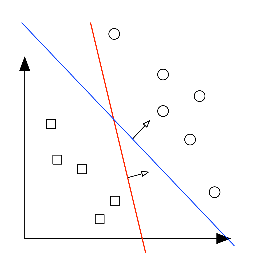
\includegraphics[width= \textwidth]{note0}
		\caption{Two different separating hyperplanes for the same data set}
		\label{fig:side:a}
	\end{minipage}
	\begin{minipage}[t]{0.4\linewidth}
		\centering
		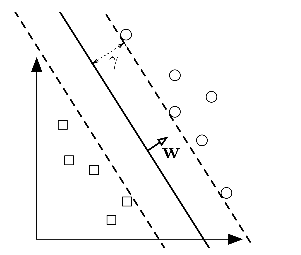
\includegraphics[width=\textwidth]{note0_2}
		\caption{The maximum margin hyperplane}	
		\label{fig:side:b}
	\end{minipage}
\end{figure}

\end{frame}

%---------------------------------------------------
\begin{frame}

\frametitle{SVM:}

\begin{block}{definition:}
\begin{itemize}
\item Data Set: \{($\mathbf{x}_{1}$,$\mathbf{x}_{1}$),($\mathbf{x}_{2}$,$\mathbf{y}_{2}$),...,($\mathbf{x}_{N}$,$\mathbf{y}_{N}$)\}
\item Binary Classification  Label: $\mathbf{y}_{i}\in \{-1,+1\}$, i=1,...,N
\item Linear Classifier: h(x) = sign($\mathbf{w}^T\mathbf{x}$+$\mathbf{b}$)
\end{itemize}
\end{block}

\begin{figure}
	\begin{minipage}[t]{0.35\linewidth}
		\centering
		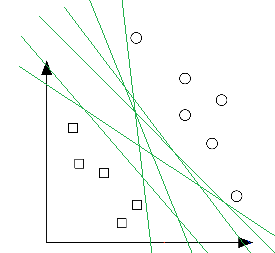
\includegraphics[width= \textwidth]{note0_1}
		\caption{Many separating hyperplanes for the same data set}
		\label{fig:side:b}
	\end{minipage}
	\hfill
	\begin{minipage}[b]{0.55\linewidth}
\quad \quad Let's review the content of the Perceptron we learned earlier.If the data is linearly separable, we can find many different hyperplanes through the Perceptron.In the left figure,we can see many diffrent separating hyperplanes for the same data.\\\\ \textcolor{red}{\LARGE A natural question to ask is:  What is the best separating hyperplane?}
	\end{minipage}
\end{figure}


\end{frame}
%---------------------------------------------------
\begin{frame}
\frametitle{SVM:}

\begin{figure}
	\begin{minipage}[t]{0.4\linewidth}
		\centering
		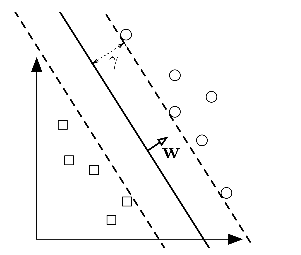
\includegraphics[width=\textwidth]{note0_2}
		\caption{The maximum margin hyperplane}	
		\label{fig:side:b}
	\end{minipage}
\end{figure}

\quad \quad {\LARGE The answer} is the one that maximizes the distance to the closest data points from both classes and we say it is the hyperplane with maximum margin. \\As show in the top figure, the margin, $\gamma$ , is the distance from the hyperplane (solid line) to the closest points in either class (which touch the parallel dotted lines).

\end{frame}

%----------------------------------------------------
\section{Linear Support Vector Machine}
%----------------------------------------------------
\subsection{Margin}

\begin{frame}
\frametitle{Margin:}
\begin{itemize}
	\item hyperplane : $\mathbf{H}$ = \{ $\mathbf{x} \vert \mathbf{w}^T\mathbf{x}$ + $\mathbf{b}$ = 0\}
	\item distance from the hyperplane to the closest point across both classes : $\gamma$
\end{itemize}


%\begin{figure}[h]
%	\centering
%	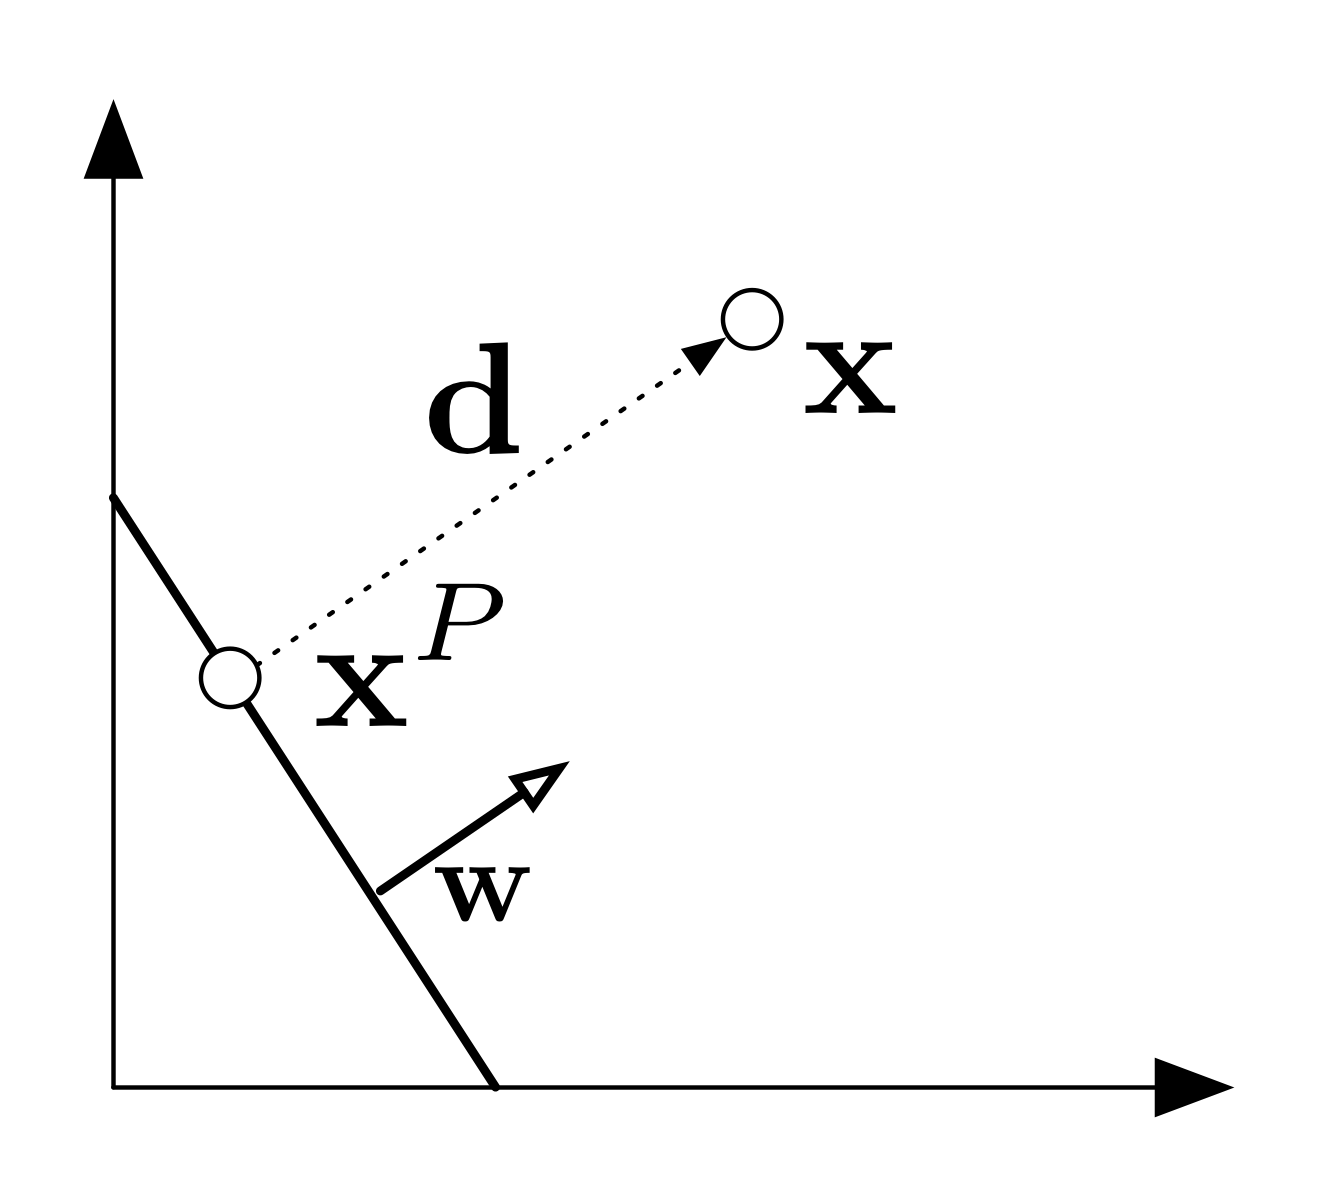
\includegraphics[scale=0.4]{projection}
%\end{figure}

\begin{figure}

	\begin{minipage}[b]{0.55\linewidth}

\begin{block}{Margin:}
\begin{spacing}{1.4}
Consider some point $\mathbf{x}$. Let $\mathbf{d}$ be the vector from $\mathbf{H}$ to $\mathbf{x}$ of minimum length.  Let $\mathbf{x}^P$ be the projection of $\mathbf{x}$  onto $\mathbf{H}$ . It follows then that: 
\centerline{ $\mathbf{x}^P = \mathbf{x} - \mathbf{d}$ }
 $\mathbf{d}$  is parallel to $\mathbf{w}$ , so $\mathbf{d}=\alpha\mathbf{w}$   for some $\alpha\in\mathbb{R}$ \\
$\mathbf{x}^P\in\mathcal{H}$ which implies $\mathbf{w}^T\mathbf{x}^P+b=0$ \\
therefore $\mathbf{w}^T\mathbf{x}^P+b=\mathbf{w}^T(\mathbf{x}-\mathbf{d})+b=\mathbf{w}^T(\mathbf{x}-\alpha\mathbf{w})+b=0 $
which implies : $\alpha=\frac{\mathbf{w}^T\mathbf{x}+b}{\mathbf{w}^T\mathbf{w}} $ \\
\end{spacing}
\end{block}

	\end{minipage}
	\hfill
	\begin{minipage}[t]{0.35\linewidth}
		\centering
		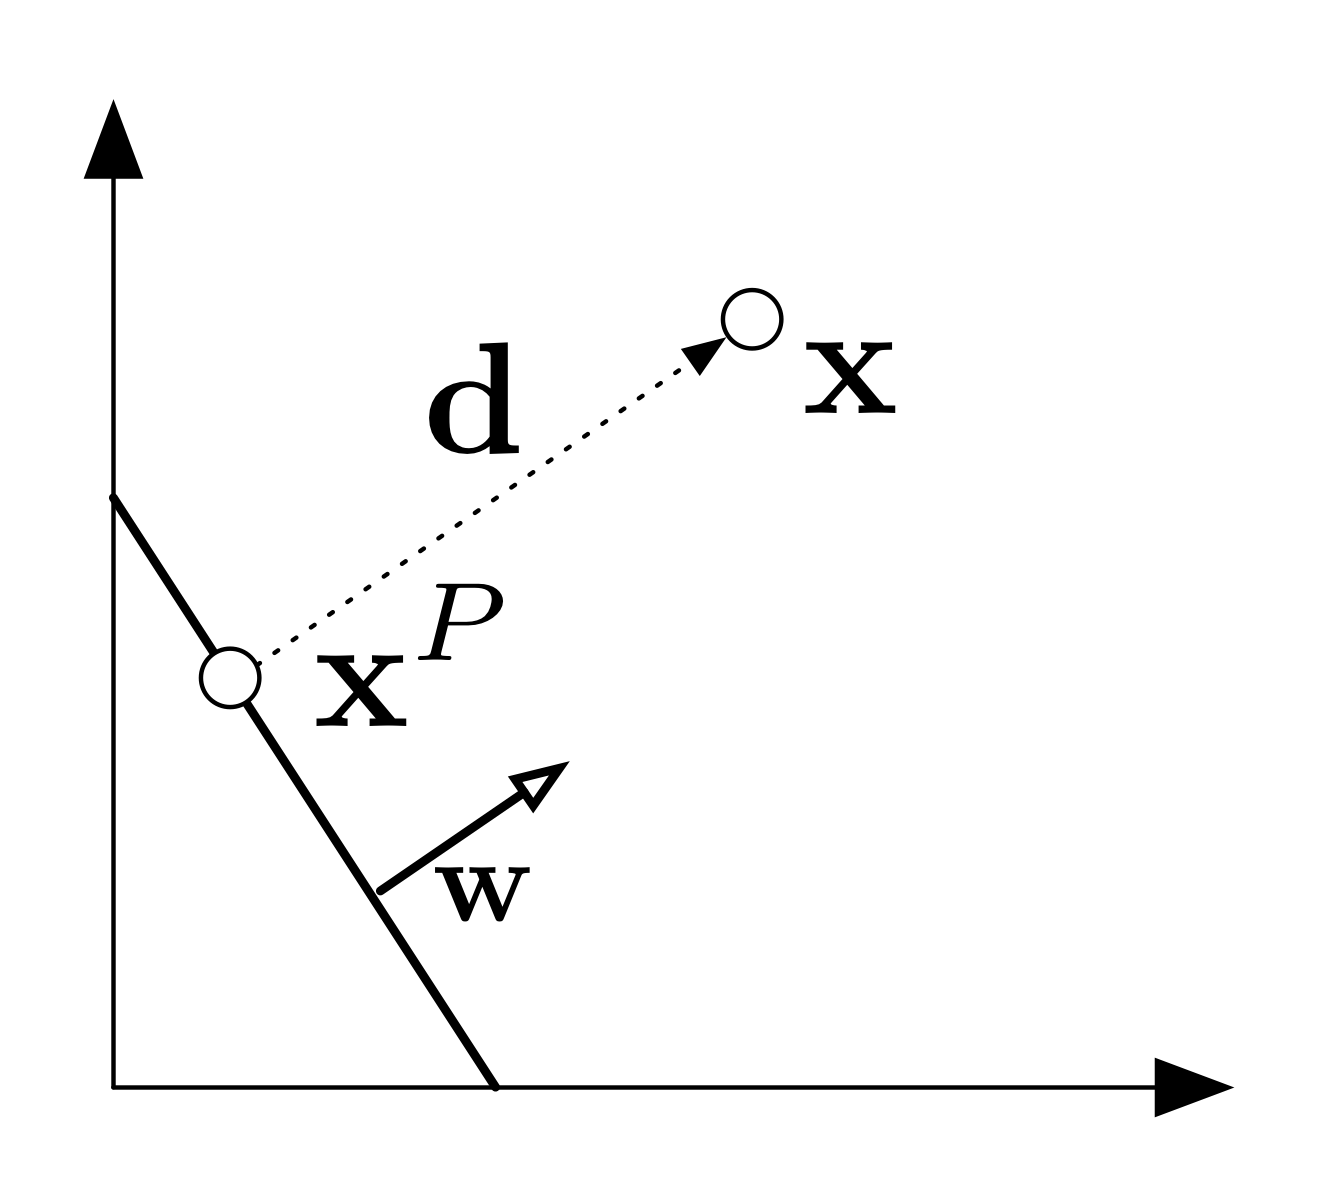
\includegraphics[width= \textwidth]{projection}
		\label{fig:side:b}
	\end{minipage}
\end{figure}

\end{frame}
%----------------------------------------------------
\begin{frame}
\frametitle{Margin:}

\begin{block}{Margin:}
\begin{spacing}{1.4}
The length of $\mathbf{d}$ : \\
\centerline { $\left \| \mathbf{d} \right \|_2=\sqrt{\mathbf{d}^T\mathbf{d}}=\sqrt{\alpha^2\mathbf{w}^T\mathbf{w}}=\frac{\left | \mathbf{w}^T\mathbf{x}+b \right |}{\sqrt{\mathbf{w}^T\mathbf{w}}}=\frac{\left | \mathbf{w}^T\mathbf{x}+b \right |}{\left \| \mathbf{w} \right \|_{2}}$ } 
Margin of  $\mathbf{H}$  with respect to $\mathbf{D}$: \centerline {$\gamma(\mathbf{w},b)=\min_{\mathbf{x}\in D}\frac{\left | \mathbf{w}^T\mathbf{x}+b \right |}{\left \| \mathbf{w} \right \|_{2}}$} \\
By definition, the margin and hyperplane are scale invariant: \centerline {$\gamma(\beta\mathbf{w},\beta b)=\gamma(\mathbf{w},b), \forall \beta \neq 0 $}
\end{spacing}
\end{block}
\[\]
\quad \quad If the hyperplane is such that $\gamma$  is maximized, it must lie right in the middle of the two classes. In other words, $\gamma$  must be the distance to the closest point within both classes. And this hyperplane is the best separating hyperplane that we want to get.

\end{frame}
%------------------------------------------------
\subsection{Max Margin Classifier}

\begin{frame}
\frametitle{Max Margin Classifier:}

\begin{spacing}{1.4}

\quad \quad We can formulate our search for the maximum margin separating hyperplane as a constrained optimization problem. The objective is to maximize the margin under the constraints that all data points must lie on the correct side of the hyperplane:
\begin{spacing}{2.0}
\centerline { $ \underbrace{\max_{\mathbf{w},b}\gamma(\mathbf{w},b)}_{maximize \ margin}  \textrm{such that} \ \  \underbrace{\forall i \ y_{i}(\mathbf{w}^Tx_{i}+b)\geq 0}_{separating \ hyperplane} $}
\end{spacing}

If we plug in the definition of $\gamma$  we obtain : 
\begin{spacing}{2.0}
\centerline { $ \underbrace{\max_{\mathbf{w},b}\underbrace{\frac{1}{\left \| \mathbf{w} \right \|}_{2}\min_{\mathbf{x}_{i}\in D}\left | \mathbf{w}^T\mathbf{x}_{i}+b \right |}_{\gamma(\mathbf{w},b)} \ }_{maximize \ margin} \ \  s.t. \ \  \underbrace{\forall i \ y_{i}(\mathbf{w}^Tx_{i}+b)\geq 0}_{separating \ hyperplane} $ }
\end{spacing}

\end{spacing}
\end{frame}

%------------------------------------------------
\begin{frame}
\frametitle{Max Margin Classifier:}

\begin{spacing}{1.4}

\quad \quad Because the hyperplane is scale invariant, $\gamma(\beta\mathbf{w},\beta b)=\gamma(\mathbf{w},b), \forall \beta \neq 0 $ , we can fix the scale of $\mathbf{w},b$  anyway we want. So we can make it such follows for simpler : 
\begin{spacing}{2.0}
\centerline { $ \min_{\mathbf{x}\in D}\left | \mathbf{w}^T\mathbf{x}+b \right |=1.$}
\end{spacing}

We can add this re-scaling as an equality constraint. Then our objective becomes:
\begin{spacing}{2.0}
\centerline { $ \max_{\mathbf{w},b}\frac{1}{\left \| \mathbf{w} \right \|_{2}}\cdot 1 = \min_{\mathbf{w},b}\left \| \mathbf{w} \right \|_{2} = \min_{\mathbf{w},b} \mathbf{w}^\top \mathbf{w} $ }
\end{spacing}

So from the objective above wo know that convex quadratic function.

\end{spacing}
\end{frame}
%------------------------------------------------

%------------------------------------------------
\begin{frame}
\frametitle{Max Margin Classifier:}

\begin{spacing}{1.4}

From above discussed, our new optimization problem becomes: 
%$ \min_{\mathbf{w},b} \mathbf{w}^\top\mathbf{w}  $
\begin{spacing}{2.0}
%\begin{align}
\centerline{ $ \min_{\mathbf{w},b} \mathbf{w}^\top\mathbf{w}  $ }
\centerline{\textrm{s.t. } $ \forall i,  y_{i}(\mathbf{w}^T \mathbf{x}_{i}+b) \geq 0 $ , 
 $\min_{i}\left | \mathbf{w}^T \mathbf{x}_{i}+b \right  | = 1$ }
\end{spacing}

And then we can merge the constraints and get a much simpler formulation : 
\begin{spacing}{2.0}
\centerline{ $ \min_{\mathbf{w},b} \mathbf{w}^\top\mathbf{w}  $ }
\centerline { \textrm{s.t.} \ \ \ $\forall i \ y_{i}(\mathbf{w}^T \mathbf{x}_{i}+b) \geq 1 $}

\end{spacing}

\quad \quad This new formulation is a quadratic optimization problem. The objective is quadratic and the constraints are all linear. We can be solve it efficiently with any QCQP (Quadratically Constrained Quadratic Program) solver.\\
\quad \quad With hyperplane scale invariant we can find the simplest hyperplane (where simpler means smaller $ \mathbf{w}^\top\mathbf{w}$ ) such that all inputs lie at least 1 unit away from the hyperplane on the correct side. 

\end{spacing}
\end{frame}
%------------------------------------------------
\subsection{Support Vectore}

\begin{frame}
\frametitle{Support Vectors:}

\begin{figure}[h]
	\centering
	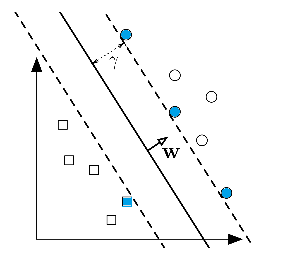
\includegraphics[scale = 0.7]{note1_2}
\end{figure}

\quad \quad Because the hyperplane is scale invariant,so we can re-scale $\mathbf{w}$,b to make the distance of all points at least 1 unit. Thus, for the optimal  $\mathbf{w}$,b  pair, some training points will have tight constraints, i.e.
\centerline{ $ y_{i}(\mathbf{w}^T \mathbf{x}_{i}+b) = 1.  $ } \\
\quad \quad In the top figure we can clearly see these points are the blue pointse and they are on the dotted lines. We refer to these training points as {\LARGE support vectors}. Support vectors are special because they are the training points that define the maximum margin of the hyperplane to the data set and they therefore determine the shape of the hyperplane. If you were to move one of them and retrain the SVM, the resulting hyperplane would change.


\end{frame}

%------------------------------------------------
\subsection{Example of SVM}

\begin{frame}
\frametitle{Example of SVM:}

\begin{figure}
	\begin{minipage}[t]{0.4\linewidth}
		\centering
		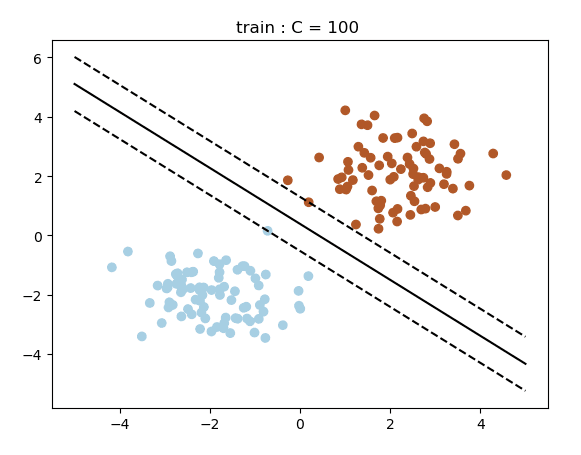
\includegraphics[width= \textwidth]{train_svm}
		\caption{train result}
		\label{fig:side:a}
	\end{minipage}
	\begin{minipage}[t]{0.4\linewidth}
		\centering
		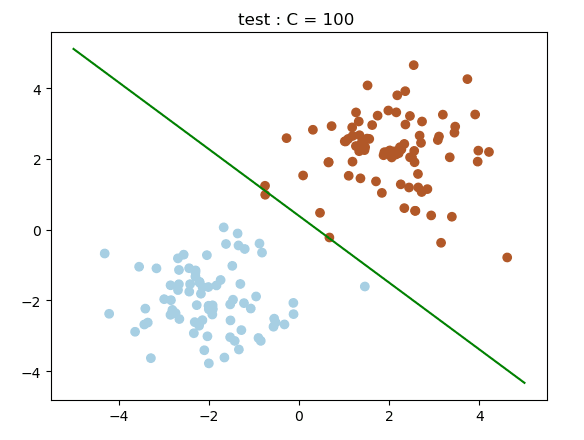
\includegraphics[width=\textwidth]{test_svm}
		\caption{test result}	
		\label{fig:side:b}
	\end{minipage}
\end{figure}


\par \quad 
\par \quad 
\centerline{\textcolor{blue}{\LARGE \href{testSVM.py}{SVM code click here} } }



\end{frame}


%------------------------------------------------
\section{SVM with soft constraints}
%------------------------------------------------
\subsection{Soft SVM Overview}

\begin{frame}
\frametitle {Soft SVM Overview:}

{\large \quad \quad  If the data is low dimensional or some noise in the data it is often the case that there is no separating hyperplane between the two classes or the result of SVM may overfit.}

\begin{figure}
	\centering
	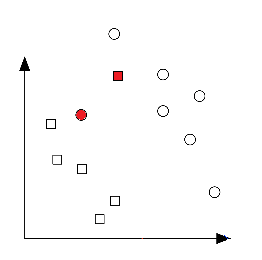
\includegraphics[scale=0.7]{note_wrong0}
	\caption{Not Linear Separate}
	\label{fig:side:a}
\end{figure}

\begin{spacing}{1.4}
\quad \quad  For example, in the top figure, the red points may be noise points or the label of the points is wrong, it's obvious that there is no solution to the optimization problems stated above.
\end{spacing}

\end{frame}

%------------------------------------------------

\begin{frame}

\frametitle {Soft SVM Overview:}

\begin{figure}
	\centering
	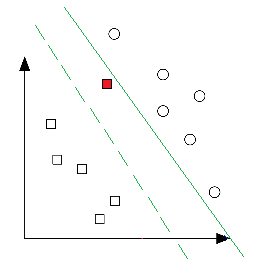
\includegraphics[scale=0.7]{note_wrong3}
	\caption{May Contain Noise}
	\label{fig:side:a}
\end{figure}

\begin{spacing}{1.4}
\quad \quad For this case , in the top figure,we can find a linear separating hyperplane(solid line) with the solution stated above. But this hyperplane's margin to the point is too small. Thus, we may think the red point is noise or the label is wrong. If we don't consider the red point, we may find the other better hyperplane(dotted line) and this may be the best hyperplane.
\end{spacing}

\end{frame}

%------------------------------------------------
\subsection{Unconstrained Formulation}

\begin{frame}
\frametitle{Unconstrained Formulation:}

\begin{spacing}{1.4}

\begin{block}{misMatched Count Loss}
\quad \quad For the case discussed above, we can ignore these noise points that mismatched and treat them as a loss. We count the number of mismatched points and add them to objective. We will get : 

\begin{spacing}{1.0}
\centerline { $\min_{\mathbf{w},b}\mathbf{w}^T\mathbf{w}+C\sum_{i=1}^{n} [ y_{n} \neq  sign(\mathbf{w}^T\mathbf{x}+\mathbf{b}) ]$ } 
%\centerline {  s.t. $ \ y_{i}(\mathbf{w}^T\mathbf{x}_{i}+b)\geq 1 $}      
\begin{equation}
	s.t.
	\begin{array}{lr}
		\ y_{i}(\mathbf{w}^T\mathbf{x}_{i}+b)\geq 1 ,        & { if \  y_{i} \  is \  correct} \\
		\ y_{i}(\mathbf{w}^T\mathbf{x}_{i}+b)\geq - \infty , & { if \  y_{i} \  is \  incorrect} \\
	\end{array}
\end{equation}
\end{spacing}
\end{block}
\quad \quad From the constration(1) , if $y_{i}$ is incorrect, we donot add any constrations to the noise points. And in the objective above, C is trade-off of \textbf{large margin} \& \textbf{noise tolerance}. \\



\end{spacing}
\end{frame}

%------------------------------------------------
\begin{frame}
\frametitle {Unconstrained Formulation:}

\begin{spacing}{1.4}
\quad \quad In the last page, we define the misMatched count loss, \textbf{[$\centerdot$]} to count the number of mismatched. However it is non-linear and discontinuous. This is very inconvenient for our calculations. Thus, we can fix that by using a linear constraints slack variables $\xi _{i}$ recorded 'margin violation' instead of the mismatched count:

\begin{spacing}{2.0}
\centerline { $\min_{\mathbf{w},b}\mathbf{w}^T\mathbf{w}+C\sum_{i=1}^{n}\xi _{i}$ } 
\centerline {  s.t. $\forall i \ y_{i}(\mathbf{w}^T\mathbf{x}_{i}+b)\geq 1-\xi_i \  , \forall i \ \xi_i \geq 0 $}       
\end{spacing}

\quad \quad The slack variable $\xi_i$   allows the input $\mathbf{x}_i $   to be closer to the hyperplane (or even be on the wrong side), but there is a penalty in the objective function for such "slack". If C is very large, the SVM becomes very strict and tries to get all points to be on the right side of the hyperplane. If C is very small, the SVM becomes very loose and may "sacrifice" some points to obtain a simpler (i.e. lower $\|\mathbf{w}\|_2^2 $  ) solution. We will get examples in next section.

\end{spacing}

\end{frame}

%------------------------------------------------

\begin{frame}

\frametitle{Unconstrained Formulation: }

\begin{block}{Loss $\xi_i$}

\begin{spacing}{1.4}
Let us consider the value of $\xi_i$   for the case of C $\neq$ 0 . We can consider $\xi_i$ as the loss and the objective will always try to minimize $\xi_i$   as much as possible, the equation must hold as an equality and we have:\\

\begin{equation}
\xi_i = \left\{
	\begin{array}{lr}
		1-y_{i}(\mathbf{w}^T \mathbf{x}_{i}+b) , & { if \  y_{i}(\mathbf{w}^T \mathbf{x}_{i}+b)<1} \\
		 0, & { if \  y_{i}(\mathbf{w}^T \mathbf{x}_{i}+b)\geq 1}.\\
	\end{array}
\right.
\end{equation}

This is equivalent to the following closed form: \\
\centerline { $\xi_i=\max(1-y_{i}(\mathbf{w}^T \mathbf{x}_{i}+b) ,0). $ }

\end{spacing}
\end{block}

\end{frame}

%------------------------------------------------

\begin{frame}
\frametitle{Unconstrained Formulation: }
\begin{block}{Unconstrained Formulation}

\begin{spacing}{1.4}
If we plug this closed form into the objective of our SVM optimization problem, we obtain the following unconstrained version as loss function and regularizer: 

\begin{spacing}{2.0}
\centerline { $ \min_{\mathbf{w},b}\underbrace{\mathbf{w}^T\mathbf{w}}_{l_{2}-regularizer}+        C\  \sum_{i=1}^{n}\underbrace{\max\left [ 1-y_{i}(\mathbf{w}^T \mathbf{x}+b),0 \right ]}_{hinge-loss}        	\label{eq:svmunconst} $ }
\end{spacing}

\quad \quad This formulation allows us to optimize the SVM paramters ($\mathbf{w},b$  ) just like logistic regression (e.g. through gradient descent). The only difference is that we have the \textbf{hinge-loss} instead of the \textbf{logistic loss}. 

\end{spacing}
\end{block}

\end{frame}

%------------------------------------------------
\subsection {Eaxmple of Soft SVM }

\begin{frame}
\frametitle{Example of Soft SVM : }

\begin{figure}
	\begin{minipage}[t]{0.3\linewidth}
		\centering
		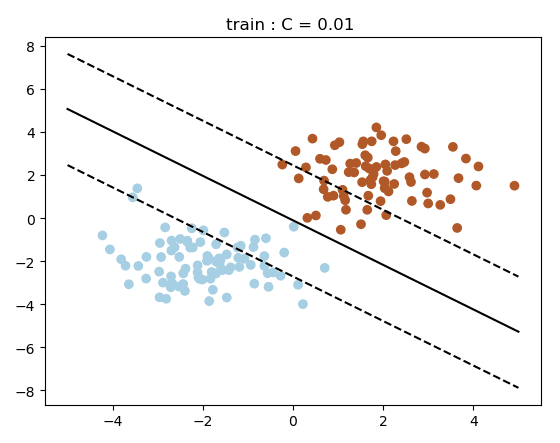
\includegraphics[width= \textwidth]{eg1_train}
		\caption{train : C=0.01}
		\label{fig:side:a}
	\end{minipage}
	\begin{minipage}[t]{0.3\linewidth}
		\centering
		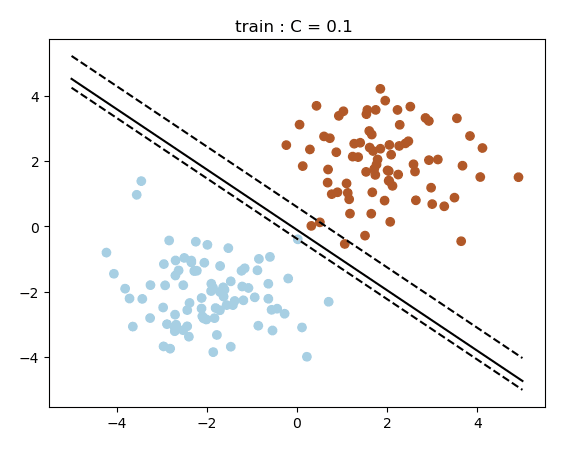
\includegraphics[width=\textwidth]{eg2_train}
		\caption{train : C=0.1}	
		\label{fig:side:b}
	\end{minipage}
	\begin{minipage}[t]{0.3\linewidth}
		\centering
		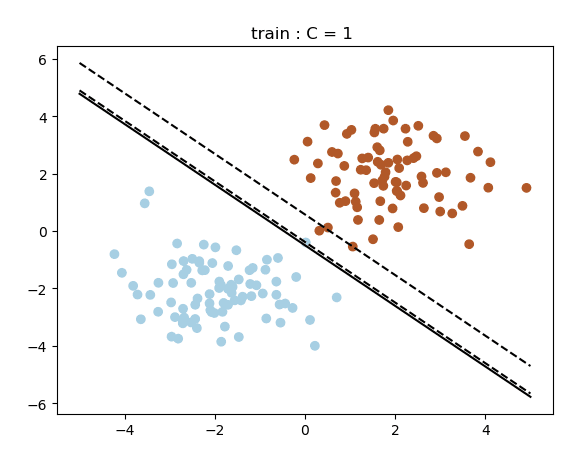
\includegraphics[width=\textwidth]{eg3_train}
		\caption{train : C=1}	
		\label{fig:side:b}
	\end{minipage}

	\begin{minipage}[t]{0.3\linewidth}
		\centering
		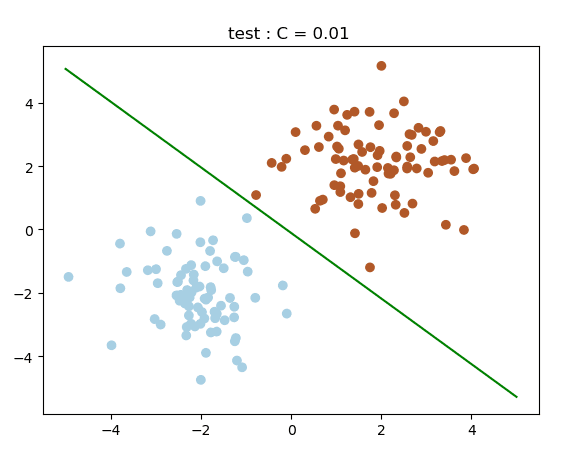
\includegraphics[width= \textwidth]{eg1_test}
		\caption{test : C=0.01}
		\label{fig:side:a}
	\end{minipage}
	\begin{minipage}[t]{0.3\linewidth}
		\centering
		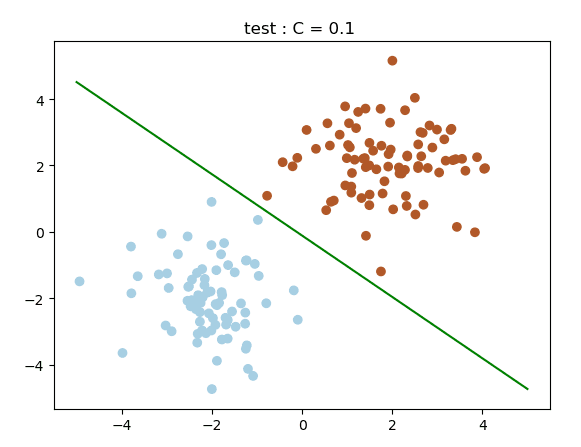
\includegraphics[width=\textwidth]{eg2_test}
		\caption{test : C=0.1}	
		\label{fig:side:b}
	\end{minipage}
	\begin{minipage}[t]{0.3\linewidth}
		\centering
		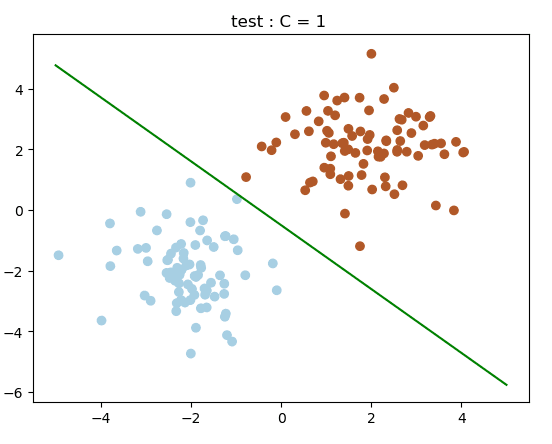
\includegraphics[width=\textwidth]{eg3_test}
		\caption{test : C=1}	
		\label{fig:side:b}
	\end{minipage}
\end{figure}

\end{frame}
%------------------------------------------------
\begin{frame}
\frametitle{Example of Soft SVM : }

\begin{figure}
	\begin{minipage}[t]{0.3\linewidth}
		\centering
		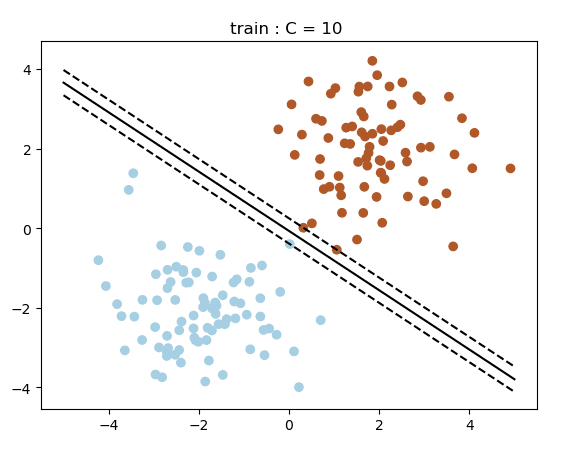
\includegraphics[width=\textwidth]{eg4_train}
		\caption{train : C=10}	
		\label{fig:side:b}
	\end{minipage}
	\begin{minipage}[t]{0.3\linewidth}
		\centering
		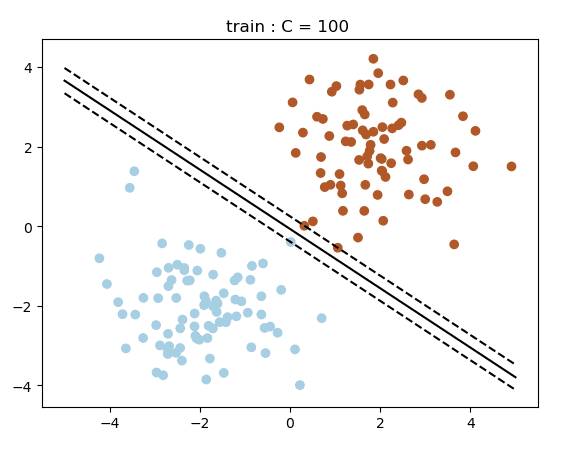
\includegraphics[width=\textwidth]{eg5_train}
		\caption{train : C=100}	
		\label{fig:side:b}
	\end{minipage}
	
	\begin{minipage}[t]{0.3\linewidth}
		\centering
		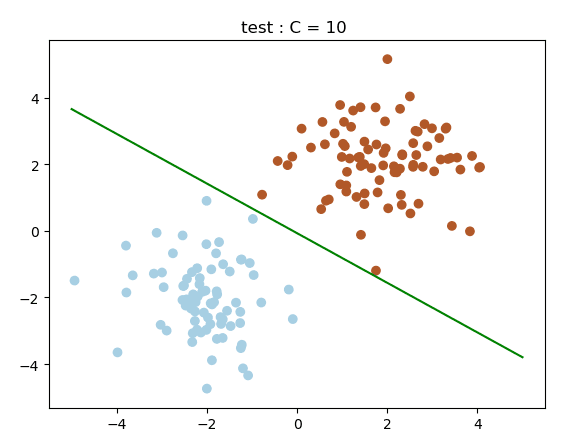
\includegraphics[width=\textwidth]{eg4_test}
		\caption{test : C=10}	
		\label{fig:side:b}
	\end{minipage}
	\begin{minipage}[t]{0.3\linewidth}
		\centering
		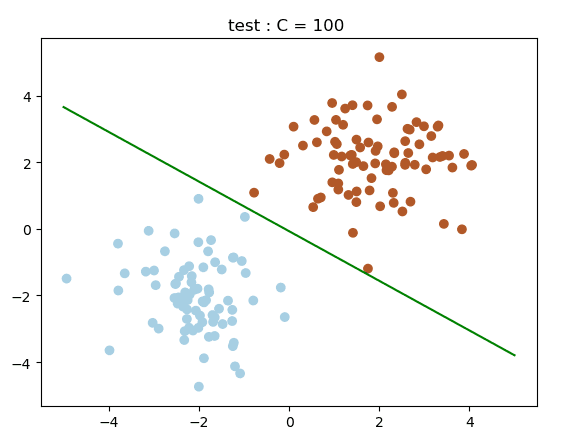
\includegraphics[width=\textwidth]{eg5_test}
		\caption{test : C=100}	
		\label{fig:side:b}
	\end{minipage}
\end{figure}

\end{frame}

%------------------------------------------------
\begin{frame}
\frametitle{Example of Soft SVM : }

\begin{spacing}{1.4}
\quad \quad From the figures above, we can see different C may get different separating hyperplane. If C is very large, the SVM becomes very strict and tries to get all points to be on the right side of the hyperplane. But it may cause overfit. If C is very small, the SVM becomes very loose and may "sacrifice" some points to obtain a simpler (i.e. lower $\|\mathbf{w}\|_2^2 $  ) solution.
\end{spacing}

\par \quad
\par \quad 
\par \quad 
\centerline{\textcolor{blue}{\LARGE \href{testSoftSVM.py}{Soft SVM code click here}} }


\end{frame}
%------------------------------------------------
\section{SVM summary}
%------------------------------------------------
\begin{frame}
\frametitle{SVM summary:}

\begin{spacing}{1.4}

\begin{itemize}
	\item The Support Vector Machine (SVM) is a linear classifier that can be viewed as an extension of the Perceptron. And SVM finds the maximum margin separating hyperplane.
	\item Margin is the distance from the hyperplane to the closest point across both classes. 
	\item Max margin clissifier is to maximize the margin under the constraints that all data points must lie on the correct side of the hyperplane.
	\item For the optimal  $\mathbf{w}$,b  pair, some training points will have tight constraints, i.e. $ y_{i}(\mathbf{w}^T \mathbf{x}_{i}+b) = 1.$ We refer to these training points as \textbf{support vectors}.
	\item That SVMs are convex quadratic function and can be solved with QCQP solver.
	\item With slack variables added into the objective, we can get the unconstrained SVM formulation : SVM with soft constraints.
\end{itemize}

\end{spacing}

\end{frame}


%------------------------------------------------
\begin{frame}
\Huge{\centerline{The End}}
\end{frame}
%------------------------------------------------

\end{CJK*}
\end{document}
%\end{document}
